

\begin{frame}[fragile]{GPU Programming Frameworks}
 \begin{center}
  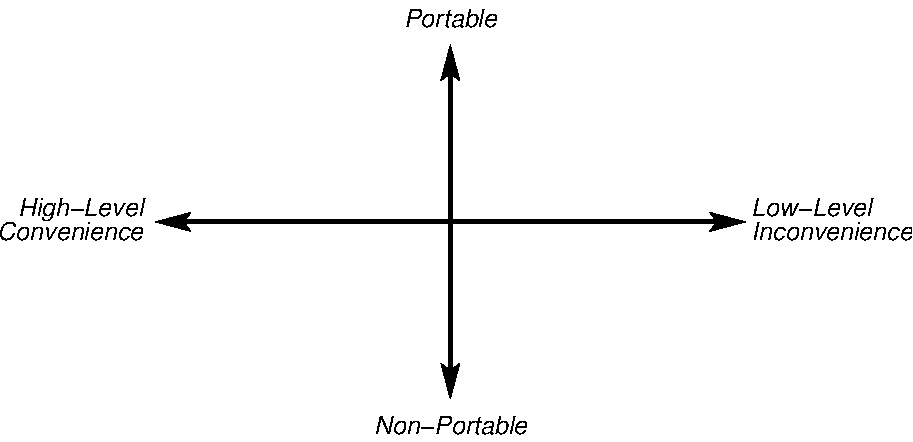
\includegraphics[width=\textwidth]{figures/gpu-programming-comparison}
 \end{center}
\end{frame}

\begin{frame}[fragile]{GPU Programming Frameworks}
 \begin{center}
  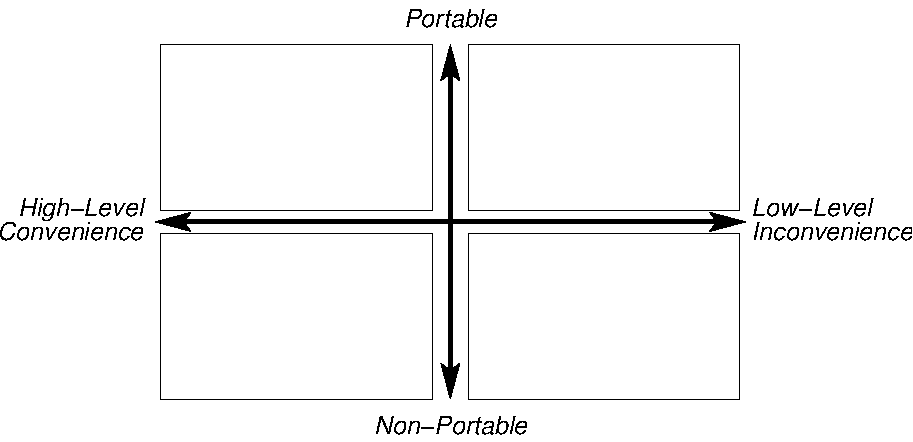
\includegraphics[width=\textwidth]{figures/gpu-programming-comparison-1}
 \end{center}
\end{frame}

\begin{frame}[fragile]{GPU Programming Frameworks}
 \begin{center}
  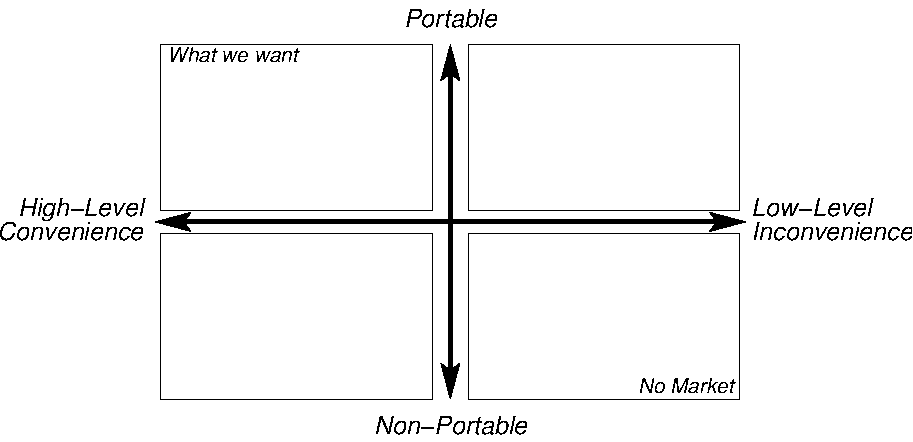
\includegraphics[width=\textwidth]{figures/gpu-programming-comparison-1a}
 \end{center}
\end{frame}

\begin{frame}[fragile]{GPU Programming Frameworks}
 \begin{center}
  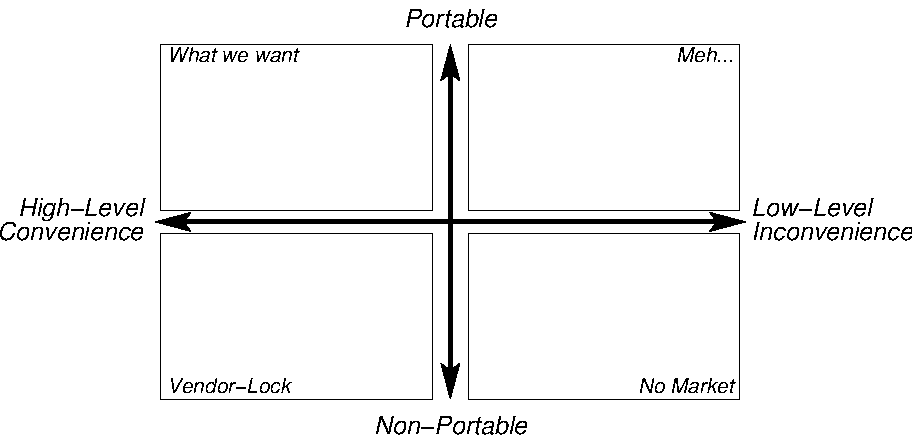
\includegraphics[width=\textwidth]{figures/gpu-programming-comparison-2}
 \end{center}
\end{frame}


\begin{frame}[fragile]
\frametitle{GPU Programming Frameworks}
 \begin{block}{NVIDIA CUDA}
  \begin{lstlisting}
// GPU kernel:
__global__ void kernel(double *buffer)
{
  int idx = blockIdx.x * blockDim.x + threadIdx.x;
  buffer[idx] = 42.0;
}

// host code:
int main()
{ 
  ...
  cudaMalloc((void**)&buffer,size);
  kernel<<<blocknum, blockdim>>>(buffer);
  ...
}
  \end{lstlisting} 

  \begin{itemize}
   \item {\color{darkgreen}Convenient}: Almost no additional code required
   \item {\color{darkred}Non-Portable}: Vendor-lock
   \item {\color{darkred}Non-Portable}: Relies on \lstinline|nvcc| being available
  \end{itemize}
 \end{block}

\end{frame}



\begin{frame}[fragile]
\frametitle{GPU Programming Frameworks}
 \begin{block}{NVIDIA CUDA Driver API}
  \begin{lstlisting}
// host code:
int main()
{ 
  ...  
  cudaMalloc((void**)&buffer,size);
  void *args[1] = { &buffer };
  cuModuleLoad(&module, module_file);
  cuModuleGetFunction(&function, module, kernel_name);
  cuLaunchKernel(function, 
                 N, 1, 1, // Nx1x1 blocks
                 1, 1, 1, // 1x1x1 threads
                 0, 0, args, 0)
  ...
}
  \end{lstlisting} 

  \begin{itemize}
   \item {\color{darkgreen}Relief}: No dependency on \lstinline|nvcc|
   \item {\color{darkred}Inconvenient}: Pseudo-Assembly PTX code
   \item {\color{darkred}Non-Portable}: PTX updated with each device generation
  \end{itemize}
 \end{block}

\end{frame}

\begin{frame}[fragile]
\frametitle{GPU Programming Frameworks}
 \begin{block}{NVIDIA CUDA Driver API}
  \begin{lstlisting}
// Generated by NVIDIA NVVM Compiler
// Compiler built on Sun Aug 19 23:20:45 2012
// Driver 304.43

.version 3.0
.target sm_13, texmode_independent
.address_size 32

.entry _k0(
 .param .u32 .ptr .global .align 4 _k0_param_0,
 .param .u32 _k0_param_1,
 .param .u32 .ptr .global .align 4 _k0_param_2,
 .param .u32 _k0_param_3,
 .param .u32 .ptr .global .align 4 _k0_param_4,
 .param .u32 _k0_param_5,
 .param .u32 _k0_param_6,
 .param .u32 _k0_param_7,
 .param .u32 .ptr .global .align 4 _k0_param_8,
 .param .u32 _k0_param_9,
 ...
)
  \end{lstlisting} 
 \end{block}

\end{frame}



\begin{frame}[fragile]
\frametitle{GPU Programming Frameworks}
 \begin{block}{OpenACC and Friends}
  \begin{lstlisting}
void func(...) {
  #pragma acc data pcopyin(A[0:size][0:size])
  {
    #pragma acc kernels loop
    for(int i=0; i< size; i++)
      for(int j=0; j < size; j++)
        A[i][j] = 42;
  }
}

int main()
{
  double A[1337][1337];
  func(A);
}
  \end{lstlisting}

  \begin{itemize}
   \item {\color{darkgreen}Convenient}: Simple OpenMP-type pragma annotations
   \item {\color{darkred}Non-Portable}: Compiler support?
   \item {\color{darkred}Non-Portable}: Insufficient control over memory transfers?
  \end{itemize}
 \end{block}

\end{frame}


\begin{frame}[fragile]
\frametitle{GPU Programming Frameworks}
 \begin{block}{OpenCL}
  \begin{lstlisting}
const char *kernel_string =
"__kernel void mykernel(__global double *buffer) {
  buffer[get_global_id(0)] = 42.0;
};";   

int main() {
  ...
  cl_program my_prog = clCreateProgramWithSource(
         my_context,1,&kernel_string,&source_len,&err);
  clBuildProgram(my_prog,0,NULL,NULL,NULL,NULL);
  cl_kernel my_kernel = clCreateKernel(my_prog,
                          "mykernel",&err);
  clSetKernelArg(my_kernel,0,sizeof(cl_mem),&buffer);
  clEnqueueNDRangeKernel(queue,my_kernel,1,NULL,
               &global_size,&local_size,0,NULL,NULL);
} 
  \end{lstlisting} 

  \begin{itemize}
   \item {\color{darkred}Inconvenient}: Low-level boilerplate code required
   \item {\color{darkgreen}Portable}: Broad hardware support (separate SDKs)
   \item {\color{darkred}Bad News}: No more development effort from NVIDIA
  \end{itemize}
 \end{block}

\end{frame}

\begin{frame}[fragile]{GPU Programming Frameworks}
 \begin{center}
  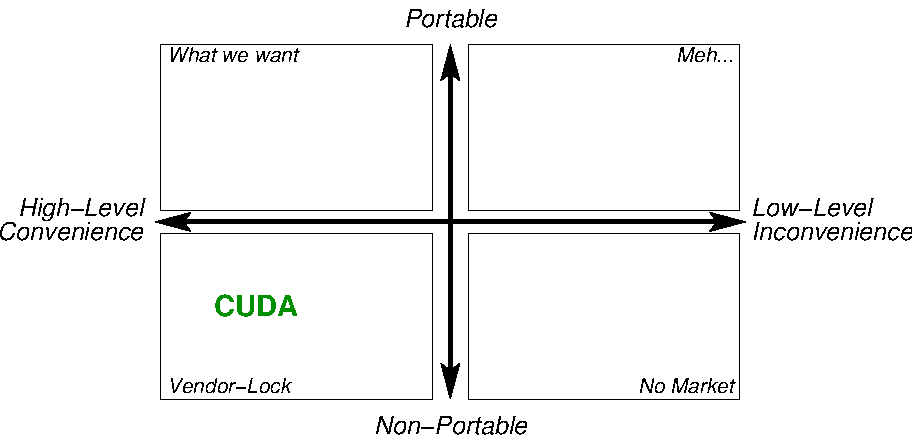
\includegraphics[width=\textwidth]{figures/gpu-programming-comparison-3}
 \end{center}
\end{frame}


\begin{frame}[fragile]{GPU Programming Frameworks}
 \begin{center}
  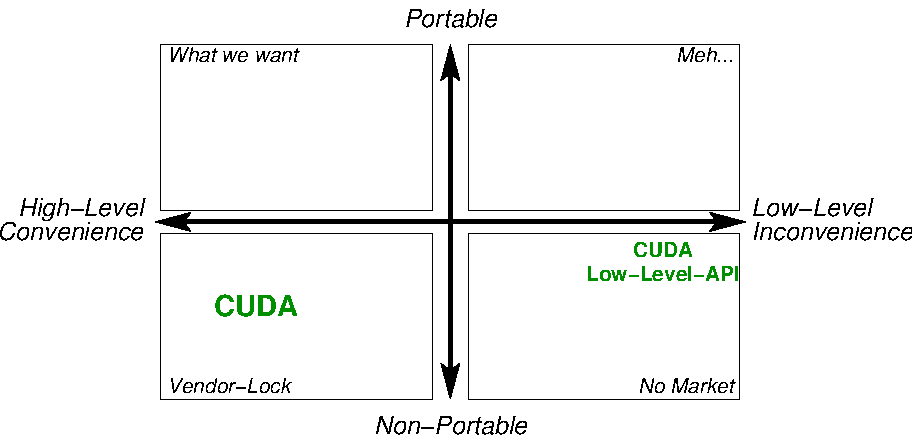
\includegraphics[width=\textwidth]{figures/gpu-programming-comparison-4}
 \end{center}
\end{frame}

\begin{frame}[fragile]{GPU Programming Frameworks}
 \begin{center}
  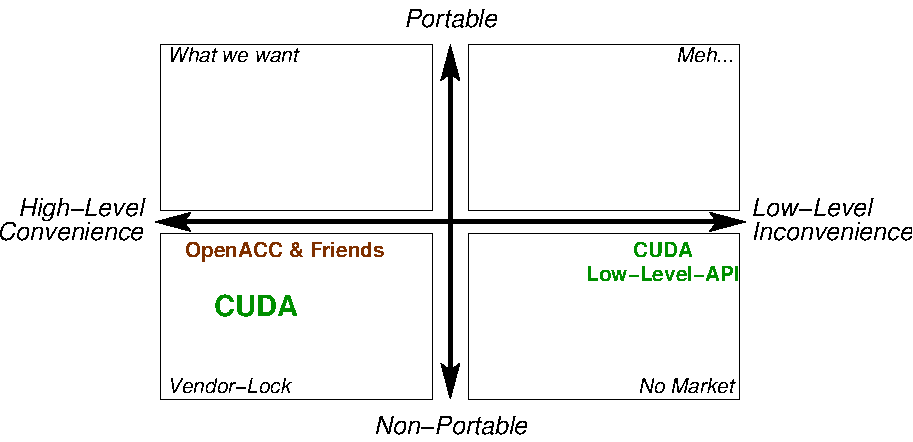
\includegraphics[width=\textwidth]{figures/gpu-programming-comparison-5}
 \end{center}
\end{frame}

\begin{frame}[fragile]{GPU Programming Frameworks}
 \begin{center}
  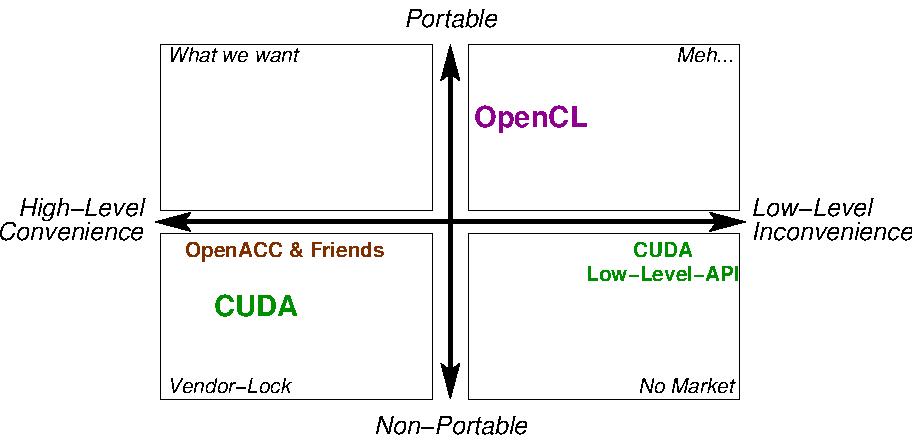
\includegraphics[width=\textwidth]{figures/gpu-programming-comparison-final}
 \end{center}
\end{frame}


\begin{frame}[fragile]
\frametitle{GPUs: Library Aspects}

 \begin{block}{Challenge: Hardware}
  \begin{itemize}
   \item Portable performance
   \item Auto-tuning
   \item Testing requires many different machines
  \end{itemize}
 \end{block}

 \begin{block}{Challenge: Memory}
  \begin{itemize}
   \item Allocation failures?
   \item Multi-GPU?
   \item PCI-Express bottleneck
  \end{itemize}
 \end{block}

 \begin{block}{Challenge: Programming}
  \begin{itemize}
   \item Kernel language?
   \item Which low-level parameters to expose?
  \end{itemize}
 \end{block}

\end{frame}


